\documentclass{article}
\setlength{\parskip}{5pt} % esp. entre parrafos
\setlength{\parindent}{0pt} % esp. al inicio de un parrafo
\usepackage{listings} % listings
\usepackage{amsmath} % mates
\usepackage[sort&compress,numbers]{natbib} % referencias
\usepackage{url} % que las URLs se vean lindos
\usepackage[top=15mm,left=20mm,right=20mm,bottom=25mm]{geometry} % margenes
\usepackage{hyperref} % ligas de URLs
\usepackage{graphicx} % poner figuras
\usepackage[spanish]{babel} % otros idiomas

\author{Claudia Lizeth Hern\'andez Ram\'irez} % author
\title{Homework 2 - Cellular Automata} % titulo
\date{\today}

\begin{document} % inicia contenido

\maketitle % cabecera

% RESUMEEEEEEEEEEEEEEEN
\begin{abstract} % resumen
  \centering
  No se encuentra un tendencia espec\'ifica de comportamiento.
  Para el rango de 0.2 a 0.5 parece como un comportamiento espec\'ifico, sin embargo como era de esperarse a valores de 0.1 y 0.9 las probabilidades infinitas son muy diferentes.
\end{abstract}


% INTRODUCCIOOOOOOOOOOOON
\section{Introducci\'{o}n}\label{intro} % seccion y etiqueta

En este trabajo se pretende establecer la posibilidad de crear vida infinita en funci\'on de la posibilidad inicial de crear vida. 




% DESARROLLOOOOOOOOOOOO
\section{Desarrollo}\label{desarrollo} % Desarrollo de la tarea
Teniendo el c\'odigo base \cite{RepoDraElisa}comenc\'e eliminando lo que no era necesario para la tarea. Posteriormente como se mencion\'o en clase necesitaba implementar dos ciclos \texttt{for} uno para variar la \texttt{p} que es la posibilidad en la que mi c\'odigo generar\'a vida por primera ocasi\'on, en mi caso decid\'i hacerlo partiendo de \texttt{0.1} hasta llegar a \texttt{0.9}; el segundo \texttt{for} era necesario para las r\'eplicas, en mi caso fueron 30 valores.

Para comenzar a determinar si quedaba alguien con vida al finalizar el c\'odigo, con la ayuda de un \texttt{if} establec\'i lo siguiente:
si mi variable \texttt{vivos} resultaba en un valor mayor a \texttt{0}, vivos tomar\'ia el valor de \texttt{1} y lo imprimir\'ia como un \texttt{1}, de lo contrario lo imprimir\'ia como un \texttt{0}.

Hasta ese momento todo parec\'ia ir bastante bien, el reto fue lograr que esos \texttt{1} y \texttt{0} se fueran contabilizando para lograr sacar la estad\'istica y probabilidad de creaci\'on de vida inifinita.
Despue\'es de dos d\'ias tratando de obtener informaci\'on y de varios intento fallidos, prob\'e con algo que me di\'o resultado.
\texttt{"datos"} representaba un data frame vac\'io.
\texttt{"unos"} y \texttt{"ceros"} eran una variable de tipo num\'erico sin un valor definido. Al terminar de ejecutarse mi \texttt{if}, llam\'e a mi variable \texttt{"unos"} y lo defin\'i como un vector el cual se conformar\'ia de la suma de los valores de \texttt{"vivos"} que fueran mayores a \texttt{0, ceros}  por otro lado har\'ia lo mismo, solo que con \texttt{"vivos"} igual a \texttt{0}.
Despu\'es imprimir\'ia mi vector \texttt{"unos"}.
Una nueva variables llamada \texttt{"dfunos"} por \texttt{"data frame unos"} entr\'o al juego, ya que ah\'i es donde se guardan mis valores de \texttt{1} y \texttt{0}.

Un nuevo problema era que no logr\'e acomodar esos valores de una manera en la que pudiera trabajar, sab\'ia c\'omo estaban constituidos, sin embargo, no logr\'e acomodarlos de una forma \'optima, por lo que se me ocurri\'o exportar a excel y acomodarlos de una mejor forma para posteriormente exportar esa misma informaci\'on a Rstudio\citep{TablasOverleaf}.
Con el paquete 'ggplot' gener\'e una gr\'afica de puntos 'geompoint' que posteriormente un\'i con un 'geomline'.

\begin{table}[ht]
    \centering
    \begin{tabular}{|c|c|c|}
         \hline
         probabilidad inicial & cantidad de unos & probabilidad inifnito\\
         \hline
         0.1 & 0.2667 & 8 \\
         \hline
         0.2 & 0.1333 & 4 \\
         \hline
         0.3 & 0.1667 & 5 \\
         \hline
         0.4 & 0.2000 & 6 \\
         \hline
         0.5 & 0.1667 & 5 \\
         \hline
         0.6 & 0.1667 & 5 \\
         \hline
         0.7 & 0.2000 & 6 \\
         \hline
         0.8 & 0.2333 & 7 \\
         \hline
         0.9 & 0.400 & 12 \\
         \hline
    \end{tabular}
    \caption{Datos que se Obtienen en Rstudio}
    \label{tab:my_label}
\end{table}
\newpage

Finalmente este es el c\'odigo con el que gener\'e toda la tarea\citep{ManualListings}:

\begin{lstlisting}
library(parallel)
library(openxlsx)
dim = 20
num = dim^2
dur = 10
p = c(0.10, 0.20, 0.30, 0.40, 0.50, 0.60, 0.70, 0.80, 0.90)
datos = data.frame()
unos = numeric()
ceros = numeric()
for (inicial in p) {
  for (replica in 1:30) { # minimo 30 1:30
    actual = matrix(round(runif(num) < p), nrow=dim, ncol=dim, byrow=TRUE) 
    paso = function(pos) {
      fila = floor((pos - 1) / dim) + 1
      columna = ((pos - 1) %% dim) + 1
      vecindad =  actual[max(fila - 1, 1) : min(fila + 1, dim), 
                         max(columna - 1, 1): min(columna + 1, dim)]
      return(1 * ((sum(vecindad) - actual[fila, columna]) == 3))
    }
    cluster <- makeCluster(detectCores() - 1)
    clusterExport(cluster, "dim")
    clusterExport(cluster, "paso")
    
    for (iteracion in 1:dur) {
      clusterExport(cluster, "actual")
      siguiente <- parSapply(cluster, 1:num, paso)
      vivos = sum(siguiente)
      cat(inicial, replica, iteracion, vivos, '\n') #concatenar
      actual <- matrix(siguiente, nrow=dim, ncol=dim, byrow=TRUE)
    }
    if (vivos > 0) {
      vivos = 1
      print(vivos)
    } else {
      vivos = 0
      print(0)
    }
    unos = c(unos, sum(vivos > 0)) #vector de 1s y 0s
    ceros = c(ceros, sum(vivos = 0))
    stopCluster(cluster)
    }
    print(unos)   
    dfunos = data.frame()
    dfunos = rbind(dfunos, unos)
}
write.xlsx(dfunos, file = "miarchivodf.xlsx")

library(ggplot2)#Grafica
library(openxlsx)
library(tidyverse)
library(dplyr)

ggplot(miarchivodf, aes(x = probini, 
                        y = probinfini)) +
  geom_line(color="blue") +
  geom_point(shape=21, color="blue", fill="blue", size=3) +
  theme_gray() + labs (x = "Probabilidad inicial de población", 
         y = "Probabilidad de crear vida infinita",
         title = "Juego de la vida")
\end{lstlisting}
\bigskip

Despu\'es de ejecutar el c\'odigo anterior, se obtuvo la siguiente gr\'afica.

\begin{figure}[h!] % figura
    \centering
    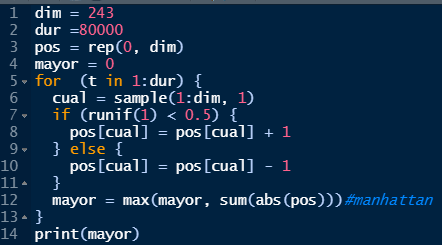
\includegraphics[width=150mm]{figura 1.PNG} % archivo
    \caption{Gr\'afica de puntos. Probabilidad de crear vida infinita.}
    \label{Figura 1}
\end{figure}
%CONCLUSIOOOON
\section{Conclusi\'on}

Con base en los resultados obtenidos en nuestra gr\'afica, podemos deducir que si comenzamos con una probabilidad inicial de poblaci\'on la probabilidad de generar vida inifnita aumenta en comparaci\'on del rango de 0.2 a 0.7, ya que sucede lo mismo en una probabilidad inicial de 0.9, en donde es casi un 50\% de probabilidad de generar vida infinita.
El comportamiento que tiene la gr\'afica no muestra tendencia general, sino que tiene altos y bajos.
\bigskip

% BIBLIOGRAFIAAAAAAS
\bibliography{referencias}
\bibliographystyle{plainnat}
\end{document}

